% !TeX spellcheck = en_US
\section{Atlassian Jira Agile}
\subsection{What does Jira Agile provide?}

Jira Agile provides task management support for the two main agile methodologies
SCRUM and Kanban. It focuses on creating and managing tasks, issues, stories,
epics and bug reports. Developers can estimate and prioritize these planning
cards. Administrators define task flow processes according to certain filters
and constraints. All developers must follow these rules afterward. The whole
Jira framework is highly adaptable and configurable to future needs, i.e. new
Kanban board columns and statuses can be defined and multiple projects can be
visualized all at once on a configurable dashboard. It also integrates with
Jira, Confluence and other development tools. 

Another feature is the integration with source code revision tools, like Git,
SVN and Bitbucket. It bridges the gap between user stories and source code
commits.

On the side of analysis, Jira Agile does not offer a lot. At least build-in features are scarce. If developers use Kanban, they can monitor current trends and analyze past progresses. The tool that visualizes this metrics is called cumulative flow diagram, please refer to figure~\ref{fig:cumulative_flow_diagram}. I think, this could be a good point where PROM comes in with analysis tools. Maybe we could add effort metrics and product metrics here. For instance, CC, LLOC, and LCOM4. It could be even feasible to integrate SonarQube features here, maybe we could add them first to PROM services, or provide an unified interface to PROM and SonarQube metrics and statistics through a REST service or something similar.

\begin{figure}[h]
	\centering
	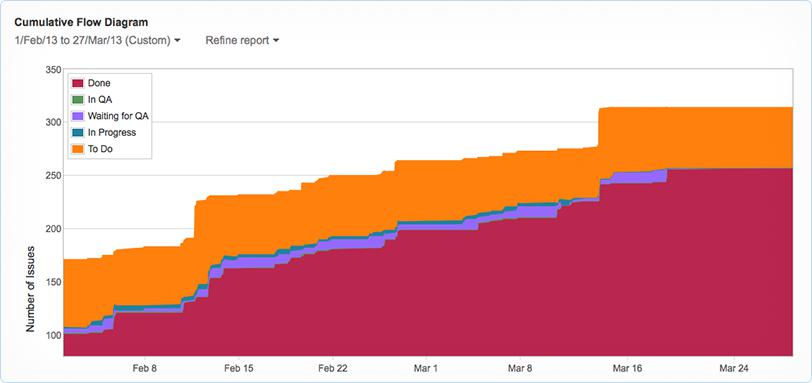
\includegraphics[scale=0.5]{img/cumulative_flow_diagram.jpg}
	\caption{Cumulative flow diagram with number of issues over time.} 
	\label{fig:cumulative_flow_diagram}
\end{figure}

Although, Atlassian Jira comes with some experimental advanced report features, that a developer can enable through a simple click. In general, users can define filters to refine charts and reports. It is possible to zoom in and out charts and move along the axis with the mouse pointer to get additional information about a certain point in time.

From our perspective, in order to add some value to these reports and charts, PROM could provide real-time effort statistics. However, I do not know now if it is possible to add functionality to these charts directly, or if it would be necessary to write a plug-in from scratch that visualizes such data enriched with our effort collections.

The following list shows the most important report types, gives a fast insight to their functionality, and screenshots. I will not provide full description to these, due to a more complete manual available online\footnote{\label{fn:report_modes}\url{https://confluence.atlassian.com/display/AGILE063/Using+Report+Mode}}. Since I am concerned about Jira Agile, I will describe only report types that match the criteria of agile methodologies. Also Jira does the same, since it excludes automatically all issues and data fields, that do not belong to a certain board type, i.e. Kanban board, and Scrum board.

The following reports and charts are available\footnoteref{fn:report_modes}:

\begin{itemize}
	\item Control Chart
	\item Burndown Chart (for Scrum boards only)
	\item Cumulative Flow Diagram
	\item Epic Report (for Scrum boards only)
	\item Sprint Report (for Scrum boards only)
	\item Velocity Chart (for Scrum boards only)
	\item Version Report (for Scrum boards only)
\end{itemize}

\textbf{Control chart}: A control chart can show the cycle time or lead time for your product, version or sprint. The horizontal x-axis in a Control Chart indicates time, and the vertical y-axis indicates the number of days issues have spent in those statuses.

\begin{figure}[h]
	\centering
	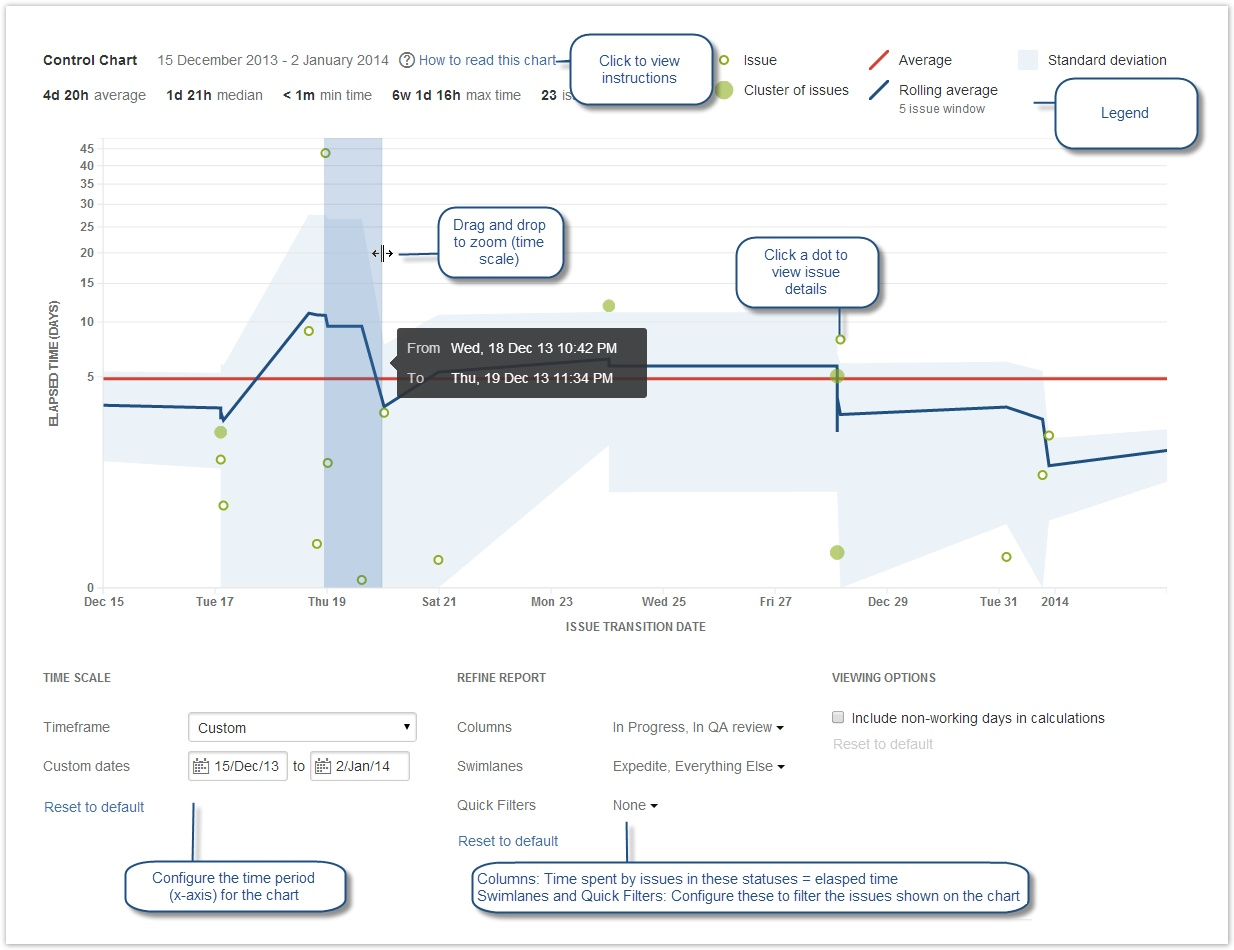
\includegraphics[scale=0.4]{img/agile-controlchart-annotated.jpg}
	\caption{Screenshot: Control Chart with annotations.} 
	\label{fig:agile-controlchart-annotated}
\end{figure}

\textbf{Burndown chart}: A Burndown Chart shows the actual and estimated amount of work to be done in a sprint. The horizontal x-axis in a Burndown Chart indicates time, and the vertical y-axis indicates cards (issues). This only applies to Scrum boards.

\begin{figure}[h]
	\centering
	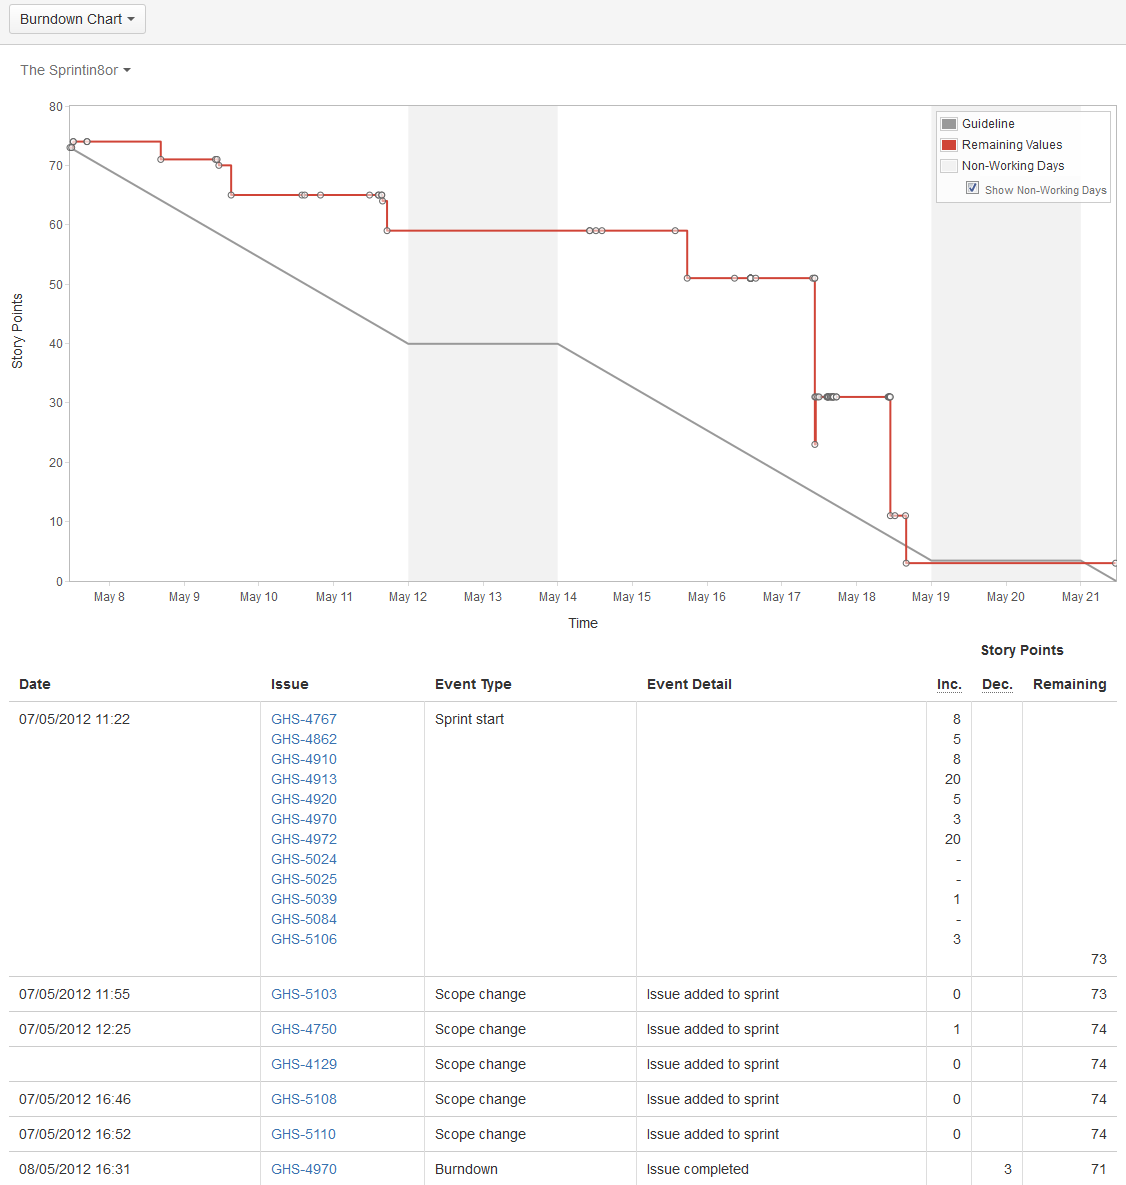
\includegraphics[scale=0.4]{img/burndown-chart.png}
	\caption{Screenshot: Burndown chart.} 
	\label{fig:burndown-chart}
\end{figure}

\textbf{Cumulative flow diagram}: A Cumulative Flow Diagram (CFD) is an area chart that shows the various statuses of work items for a product, version, or sprint. The horizontal x-axis in a CFD indicates time, and the vertical y-axis indicates cards (issues). Each colored area of the chart equates to a workflow status (i.e. a column on your board). This description is just due to completeness of content. Please refer to figure~\ref{fig:cumulative_flow_diagram} for further information.

\textbf{Epic report}: The Epic Report shows a list of complete, incomplete and unestimated issues in an epic. It is particularly useful for planning work for an epic that may extend over multiple sprints.
Use the Epic Report to understand the progress towards completing an epic over time, and to track the amount of remaining work that's incomplete or unestimated.

\begin{figure}[h]
	\centering
	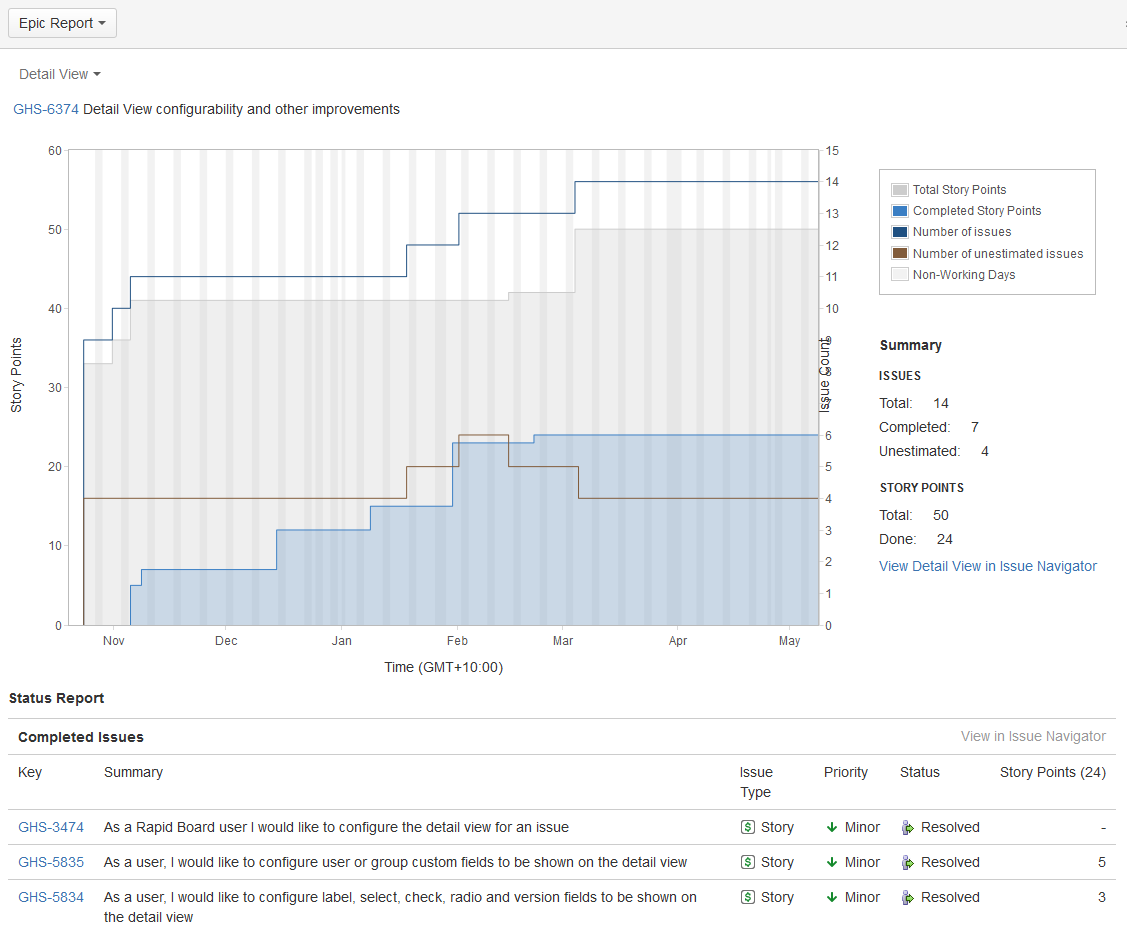
\includegraphics[scale=0.4]{img/epic-report.png}
	\caption{Screenshot: Epic report.} 
	\label{fig:epic-report}
\end{figure}

\textbf{Sprint report}: The sprint report shows the list of issues in each sprint. It is useful for your sprint retrospective meeting, and also for mid-sprint progress checks. If you have Confluence\footnote{\url{https://www.atlassian.com/software/confluence}} linked to your JIRA instance, you can also create and/or link Confluence pages to your sprint report. For example, you may want to create retrospective notes for the sprint. This only applies to Scrum boards.

\begin{figure}[h]
	\centering
	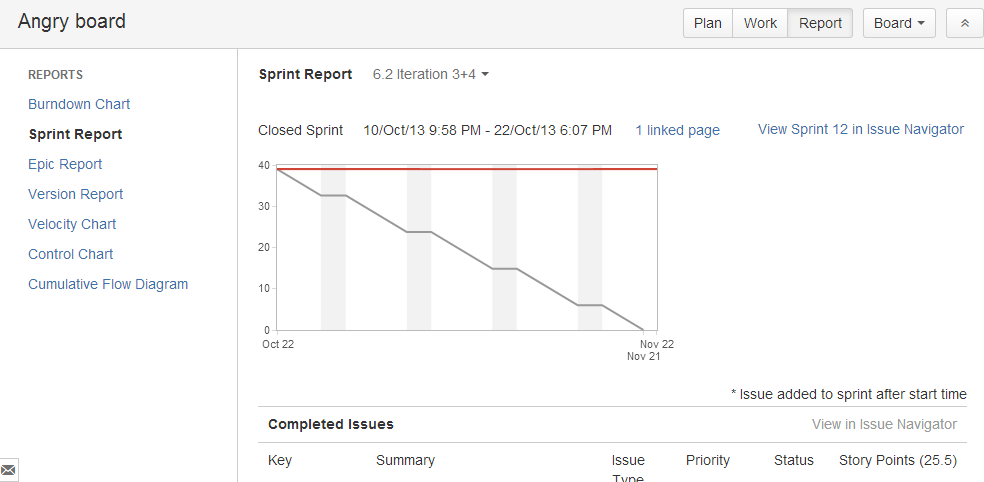
\includegraphics[scale=0.4]{img/sprintreport-linkedpages.png}
	\caption{Screenshot: Sprint report with linked Confluence pages.} 
	\label{fig:sprintreport-linkedpages}
\end{figure}

\textbf{Velocity chart}: The velocity chart shows the amount of value delivered in each sprint, enabling you to predict the amount of work the team can get done in future sprints. It is useful during your sprint planning meetings, to help you decide how much work you can feasibly commit to. This only applies to Scrum boards.

\begin{figure}[h]
	\centering
	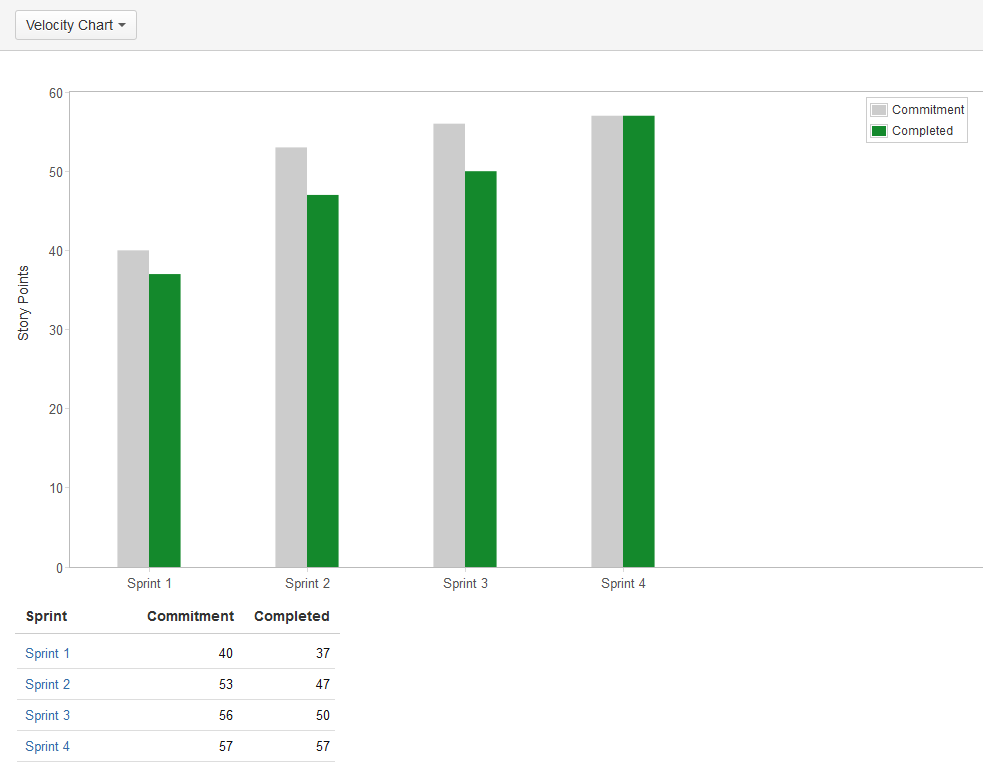
\includegraphics[scale=0.4]{img/velocity-chart.png}
	\caption{Screenshot: Velocity chart.} 
	\label{fig:velocity-chart}
\end{figure}

\textbf{Version report}: The version report shows your team's progress towards completion of a version. The version report also shows you the predicted Release Date, based on your team's average rate of progress (velocity) since the start of the version, and the estimated amount of work remaining. This only applies to Scrum boards.

\begin{figure}[h]
	\centering
	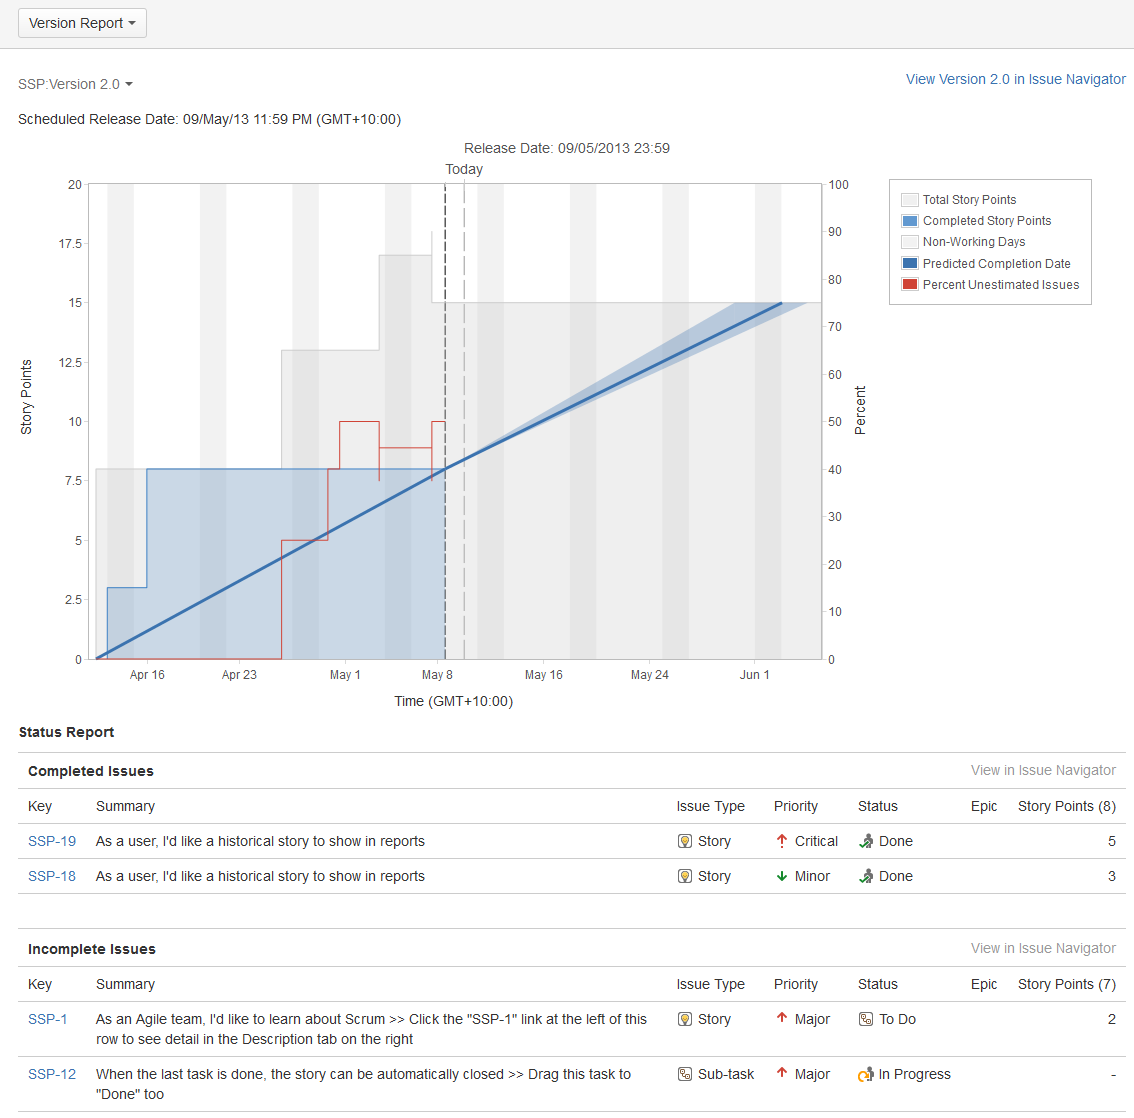
\includegraphics[scale=0.4]{img/version-report.png}
	\caption{Screenshot: Version report.} 
	\label{fig:version-report}
\end{figure}

